\documentclass[10pt]{article}

\title{ITF31519 - Portfolio, part 1, ANN}
\author{Tobias Hallingstad}

\usepackage[utf8]{inputenc}
\usepackage[english]{babel}
\usepackage{minted}
\usepackage[T1]{fontenc}

\usepackage{graphicx}

\usepackage{graphicx}
\graphicspath{ {./images/} }

\begin{document}
    \begin{titlepage}
        \maketitle
    \end{titlepage}

    \newminted{python}{
        gobble=2,
        linenos
    }

    \section{The code}
    I have decided to write the code to support 1 sett of learning data for each epoch. This is because I have the ability to ranomly create data for the ANN to learn from, using the functions \texttt{intToSplitBites(int, bits)} then \texttt{normalizeData(int, bits)}. A array of 4 elements is created in the first function, then the data is normalizes within 0 to 1 to make the ANN work. With some more work the code can support multiple setts of learning data each epoch.

    A lot of the functions use \texttt{numpy} methods. This allows the code to accept primitive data types and matrix's. 


    \section{Learning rate}
    The goal of the learning rate is to change how much the network learns. If the learning rate is small the network uses longer time to learn the correct values for the weights of the network. The goal of a learning rate is to "slow" the learning down, or speed it up. This can led to the network taking a better way to the goal.

    When the learning rate is small the network takes smaller steps each epoch of learning. This can result in the network hitting a local minimum and not reaching the correct weights to achieve the goal. For a large learning rate the network can "jump" over the optimal weights for the network, by tanking to large step.

    A good learning rate will result in the taking good time in learning the weights for the network, and get good weights at the same time.

    \section{The relationship}

    \begin{center}
        \begin{figure}[h!]
            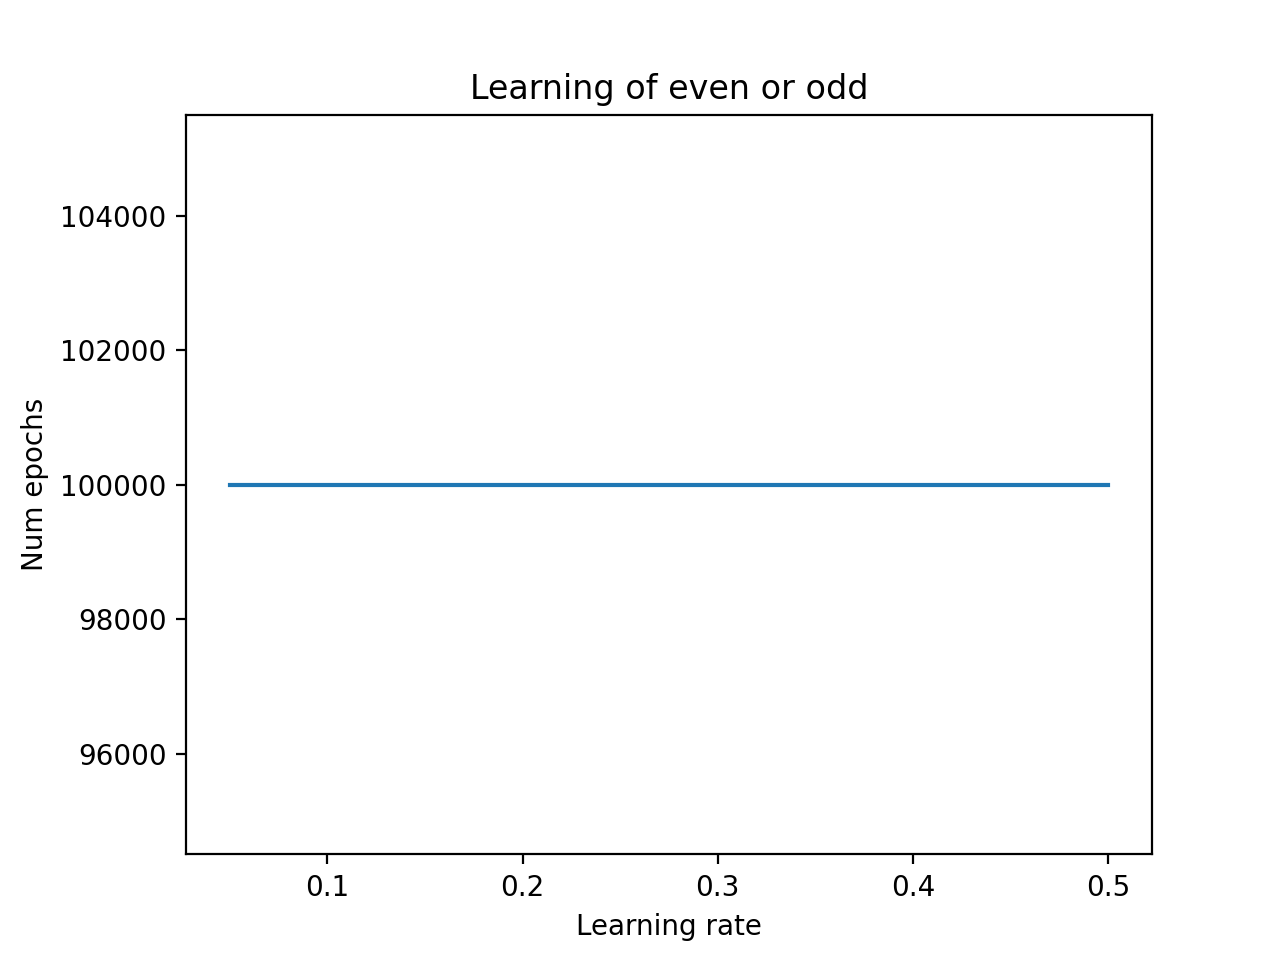
\includegraphics[scale=0.7]{Figure_1.png}
            \caption{Graph of the amount of epochs to reach an error of 0.05 with a different learning rate. Using a incomplete ANN}
        \end{figure}
    \end{center}

    I have plotted the number of epochs from 0.05 to 0.5. The graph is a line because the learning/backpropegation does not work. I have then sett a upper limit to how many loops the learning should take, and the program reaches that point. To make sure that the graph is wrong I tried to test the forward propagation with 2 numbers to se if the values move closer to some useful values.

    \begin{pythoncode}
    14: [[0.50881876]]
    15: [[0.50907909]]
    \end{pythoncode}

    This is what the forward propegation returns after 100000. The values are both close to 0.5 while 14 should be close to 0 and 15 close to 1. This is what indicates that I have a problem with the error calculation.

    If this worked as intended I would get values that are closer to 1 and 0. The amount of epochs needed to get good values for the weights would probably be around 10 000 and 100 000 at the high end. Printing the values for \texttt{W1} and \texttt{W2} gives:

    \begin{pythoncode}
    W1:
    [[0.08773227 0.82496815 0.82196337 0.74741687]
     [0.9605294  0.6102363  0.20399163 0.64866637]
     [0.47363355 0.6886396  0.0894239  0.20188402]
     [0.1869026  0.82271376 0.4024208  0.58429361]]

    W2:
    [[0.01787211]
     [0.013621  ]
     [0.0001209 ]
     [0.00097475]]
    \end{pythoncode}

    This does not give a lot of meaning, but this is what I am getting.

    \section{Final things}
    I did not get the time to compleat this task. So the implementation is incomplete. I think the problem is with how I calculate the error. This results in the ANN learning that even and odd number are around 0.5 in value, so it learns wrong. There can also be something with the backpropegation that also enforces this, but I don't have the time to test. If the learning part is fixed the rest of the code should to what the task asks, except for breaking the learning when the difference from learning and actual value is 0.05. The code is looping \texttt{r} number of times. The report is written based on what I under stand the ANN works, but I have not been able to produce the data to back up the statements.

    \subsection{Running the code}
    Just launch the file

    \subsection{GitHub}
    I have used GitHub for version control. This means that the code is accessible on GitHub. The GitHub account the code is uploaded to is Tobhal (https://github.com/Tobhal) and is my own account. 

    \section{Sources}
    All sources are linked in the \texttt{Sources.md} file.
    
\end{document}